\documentclass[xcolor=pdftex,dvipsnames,table]{beamer}
\usepackage{beamerthemesplit}
\usepackage{minted}
\usepackage{hyperref}
\usepackage{textcomp}
\usetheme{Madrid}
\usecolortheme{crane}
\title{An Alternative Introduction to Programming}
\subtitle{Read: A Tutorial of the Scheme Programming language}
\author{Shen Zheyu}
\date{\today}
\begin{document}
\maketitle
\begin{frame}[allowframebreaks]
  \frametitle{Table of Contents}
  \tableofcontents
\end{frame}
\begin{frame}
  \frametitle{Introduction}
  \begin{itemize}
    \item Shen Zheyu, sophomore ECE student
    \item My GitHub: \url{http://github.com/arsdragonfly/}
    \item SSTIA projects \url{https://github.com/SSTIA}
    %\vspace{1.3in}
  \end{itemize}
  \begin{columns}
    \begin{column}{0.5\textwidth}
      \begin{center}
        \begin{figure}
          
\includegraphics[width=0.6\textwidth]{avatar}
        \end{figure}
      \end{center}
    \end{column}
    \begin{column}{0.5\textwidth}
      \vspace*{\fill}
      \begin{center}
        \begin{figure}
          
\includegraphics[width=0.6\textwidth]{SSTIA}
        \end{figure}
      \end{center}
    \end{column}
  \end{columns}
\end{frame}
\begin{frame}[fragile]
  \frametitle{Overview}
  This seminar is intended to provide a different introduction to programming from VG101 (and arguably many other courses).
  In a (hopefully) friendly way, you'll learn many useful things unlikely to be found in other introductory material.
  \pause

  Much of the content is adapted from \textcolor{Blue}{\textit{The Little Schemer, Fourth Edition}} by D. P. Friedman and M. Felleisen.
  If you're very interested, You may also want to read \textcolor{Blue}{\textit{Structure and Interpretation of Computer Programs}} by H. Abelson and G. J. Sussman.
  \begin{center}
    \begin{figure}
      
\includegraphics[width=0.4\textwidth]{SICP.png}
    \end{figure}
  \end{center}
\end{frame}
\begin{frame}
  \frametitle{Setup}
  To begin with this seminar, you need to have a Scheme interpreter up and running.
  I personally recommend \textcolor{Blue}{Racket (\url{www.racket-lang.org})}, though other programs may also work (MIT Scheme, Guile, Chez Scheme, etc.).
\end{frame}
\begin{frame}[fragile]
  \frametitle{Setup}
  Before we start, we need to make sure that every program contains the following definitions of primitive functions:
  \begin{minted}{scheme}
  (define add1
    (lambda (n)
      (+ n 1)))
  (define sub1
    (lambda (n)
      (- n 1)))
  (define atom? (lambda (x) (not (or (pair? x) (null? x)))))
  \end{minted}
  It's recommended for this seminar now that you write your program in a single source code file, so that latter definitions of functions can build upon previous already-written ones.
\end{frame}
\begin{frame}
  \frametitle{Setup}
  \begin{center}
    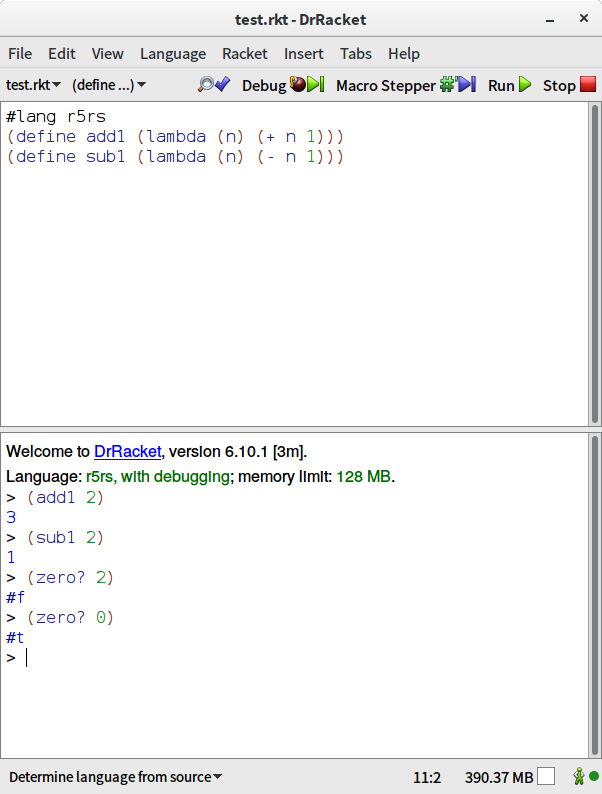
\includegraphics[height=0.8\textheight]{screenshot}
  \end{center}
\end{frame}

\section{Numbers}

\begin{frame}[fragile]
  \frametitle{Arithmetic on Natural Numbers}
    \begin{itemize}
      \item What's the answer of \mintinline{scheme}{(add1 0)}?
      \item \emph{1}.
      \pause
      \item What's the answer of \mintinline{scheme}{(sub1 3)}?
      \item \emph{2}.
      \pause
      \item What's the answer of \mintinline{scheme}{(add1 (add1 0))}?
      \item \emph{It's the answer of \mintinline{scheme}{(add1 1)}.}
      \pause
      \item What's the answer of \mintinline{scheme}{(add1 1)} then?
      \item \emph{2}.
    \end{itemize}
\end{frame}

\begin{frame}[fragile]
  \frametitle{Arithmetic on Natural Numbers}
    \begin{itemize}
      \item What's the answer of \mintinline{scheme}{(zero? 0)}?
      \item \mintinline{scheme}{#t}\emph{, which means "true".}
      \pause
      \item What's the answer of \mintinline{scheme}{(zero? 810)}?
      \item \mintinline{scheme}{#f}\emph{, which means "false".}
      \pause
      \item What's the answer of \mintinline{scheme}{(zero? (sub1 (sub1 2)))}?
      \item \mintinline{scheme}{#t}
    \end{itemize}
\end{frame}

\begin{frame}[fragile]
  \frametitle{$\lambda$ ?}
    \begin{itemize}
      \item What's the answer of \mintinline{scheme}{(lambda (x) (add1 (add1 x)))}?
      \item \emph{A \textrm{lambda expression}, which is similar to a mathematical function.}
      \pause
      \item What's the answer of \\
      \mint{scheme}{(define add2 (lambda (x) (add1 (add1 x))))}
      \mint{scheme}{(add2 (add1 3))}
      ?
      \item \emph{6.}
    \end{itemize}
\end{frame}

\begin{frame}[fragile]
  \frametitle{$\lambda$ ?}
    \begin{itemize}
      \item How does \mintinline{scheme}{(add2 (add1 3))} work?
      \item \emph{We first ask the question: what is \mintinline{scheme}{(add1 3)}?}
      \pause
      \item What is the answer of \mintinline{scheme}{(add1 3)}?
      \item \emph{4.}
      \pause
      \item What's the answer of \mintinline{scheme}{(add2 4)} then?
      \item \emph{It becomes \mintinline{scheme}{((lambda (x) (add1 (add1 x))) 4)}.}
      \pause
      \item Then?
      \item \emph{We substitute \textrm{x} for \textrm{4} in the \textrm{lambda expression}.}
      \pause
      \item What will we get then?
      \item \emph{\mintinline{scheme}{(add1 (add1 4))}}
      \pause
      \item Is that how we get 6?
      \item \emph{Yes.}
    \end{itemize}
\end{frame}

\begin{frame}[fragile]
  \frametitle{\mintinline{scheme}{cond?}}
  \begin{itemize}
    \item How does the following definition work out?
    \begin{minted}{scheme}
      (define one?
        (lambda (x)
          (cond
            ((zero? (sub1 x)) #t)
            (else #f))))
    \end{minted}
    \item \emph{We'll figure it out soon\texttrademark.}
    \pause
    \item What's the answer of \mintinline{scheme}{(one? 1)}?
    \item \mintinline{scheme}{#t}.
    \pause
    \item What's the answer of \mintinline{scheme}{(one? 2)}?
    \item \mintinline{scheme}{#f}.
  \end{itemize}
\end{frame}

\begin{frame}[fragile]
  \frametitle{\mintinline{scheme}{cond?}}
    \begin{minted}{scheme}
      (define one?
        (lambda (x)
          (cond
            ((zero? (sub1 x)) #t)
            (else #f))))
    \end{minted}
  \begin{itemize}
    \item How does the above definition work out?
  \end{itemize}
\end{frame}

\section{Lists}

\begin{frame}[fragile]
  \frametitle{Moving on to a higher order}
  \begin{itemize}
    \item What's the answer of \mintinline{scheme}{(1 2)}?
    \pause
    \item \emph{No answer. 1 is not a function that accepts 2 as an argument.}
    \pause
    \item What's the answer of \mintinline{scheme}{(foo 2)}?
    \pause
    \item \emph{No answer. \mintinline{scheme}{foo} is not a function yet.}
    \pause
    \item What's the answer of \mintinline{scheme}{(quote (1 2))}?
    \pause
    \item \emph{\mintinline{scheme}{(1 2)}}.
    \pause
    \item What's the answer of \mintinline{scheme}{'(1 2)}?
    \pause
    \item \emph{\mintinline{scheme}{(1 2)}. Same as before.}
  \end{itemize}
\end{frame}

\begin{frame}[fragile]
    \frametitle{Moving on to a higher order}
    \begin{itemize}
      \item What's the answer of \mintinline{scheme}{(atom? 1)}?
      \item \mintinline{scheme}{#t}.
      \pause
      \item What's the answer of \mintinline{scheme}{(atom? '())}?
      \item \mintinline{scheme}{#f}, \emph{because it is an empty list.}
      \pause
      \item What's the answer of \mintinline{scheme}{(atom? '(1 (2)))}?
      \item \mintinline{scheme}{#f}, \emph{because it is a list.}
      \pause
      \item What's the answer of \mintinline{scheme}{(null? '())}?
      \item \mintinline{scheme}{#f}, \emph{because it is an empty list.}
      \pause
      \item What's the answer of \mintinline{scheme}{(null? '(1 (2)))}?
      \item \mintinline{scheme}{#f}, \emph{because it is a non-empty list.}
    \end{itemize}
\end{frame}

\begin{frame}[fragile]
    \frametitle{Moving on to a higher order}
    \begin{itemize}
      \item What's the answer of \mintinline{scheme}{(car '())}?
      \item \emph{No answer, because it's an empty list.}
      \pause
      \item What's the answer of \mintinline{scheme}{(car '(1 (2)))}?
      \item \emph{1.}
      \pause
      \item What's the answer of \mintinline{scheme}{(cdr '())}?
      \item \emph{No answer, because it's an empty list.}
      \pause
      \item What's the answer of \mintinline{scheme}{(cdr '(1 (2)))}?
      \item \mintinline{scheme}{'((2))}. \emph{Note that it's different from } \mintinline{scheme}{'(2)} !
    \end{itemize}
\end{frame}

\begin{frame}[fragile]
  \frametitle{Moving on to a higher order}
  \begin{itemize}
    \item What's the answer of \mintinline{scheme}{(cons 1 '((2)))}?
    \item \emph{\mintinline{scheme}{'(1 (2))}}.
    \pause
    \item Can we build up the list from the empty list?
    \pause
    \item \emph{\mintinline{scheme}{(cons 1 (cons (cons 2 '()) '())))}}.
  \end{itemize}
\end{frame}

\begin{frame}[fragile]
  \frametitle{Moving on to a higher order}
  \begin{itemize}
    \item Define a function that removes all numbers equal to \mintinline{scheme}{x} in a list of atoms.
    \item \emph{Sure.}
  \end{itemize}
  \begin{minted}{scheme}
    (define multirember
      (lambda (x lat)
        (cond
          ((null? lat) '())
          ((= (car lat) x) (multirember x (cdr lat)))
          (else (cons (car lat) (multirember x (cdr lat)))))))
  \end{minted}
  \pause
  \begin{itemize}
    \item What are the steps to go through when dealing with a list of atoms?
    \item We always ask \mintinline{scheme}{(null? lat)} first, then ask other questions.
    \item What if we're dealing with list of lists?
    \pause
    \item We ask \mintinline{scheme}{(null? l)}, \mintinline{scheme}{(atom? (car l))} and other questions.
  \end{itemize}
\end{frame}

\begin{frame}[fragile]
  \frametitle{Moving on to a higher order}
  \begin{itemize}
    \item Could you define a function that removes all numbers less than \mintinline{scheme}{x}?
    \item \emph{Isn't this easy?}
  \end{itemize}
  \begin{minted}{scheme}
    (define multirember2
      (lambda (x lat)
        (cond
          ((null? lat) '())
          ((< (car lat) x) (multirember x (cdr lat)))
          (else (cons (car lat) (multirember x (cdr lat)))))))
  \end{minted}
\end{frame}

\begin{frame}[fragile]
  \frametitle{Moving on to a higher order}
  \begin{itemize}
    \item Could you define a function that removes all numbers greater than \mintinline{scheme}{x}?
    \item \emph{Isn't this also easy?}
  \end{itemize}
  \begin{minted}{scheme}
    (define multirember2
      (lambda (x lat)
        (cond
          ((null? lat) '())
          ((> (car lat) x) (multirember x (cdr lat)))
          (else (cons (car lat) (multirember x (cdr lat)))))))
  \end{minted}
\end{frame}

\begin{frame}[fragile]
  \frametitle{Moving on to a higher order}
  \begin{itemize}
    \item Is it really so easy as you said?
    \item \emph{What's so hard about this? we just copy the whole definition and change what we want.}
    \pause
    \item Is there a way to not copy the whole thing?
    \item \emph{What does it mean?}
    \pause
    \item Look at this function definition.
  \end{itemize}
  \begin{minted}{scheme}
(define mr-f
  (lambda (tester)
    (lambda (x lat)
      (cond
        ((null? lat) '())
        ((tester (car lat) x) ((mr-f tester) x (cdr lat)))
        (else (cons (car lat) ((mr-f tester) x (cdr lat))))))))
  \end{minted}
\end{frame}

\begin{frame}[fragile]
  \frametitle{Moving on to a higher order}
  \begin{itemize}
    \item What's the answer of \mintinline{scheme}{((mr-f =) 2 '(1 2 3))}?
    \pause
    \item \mintinline{scheme}{'(1 3)}.
    \pause
    \item What's the answer of \mintinline{scheme}{((mr-f <) 2 '(1 2 3))}?
    \pause
    \item \mintinline{scheme}{'(2 3)}.
    \pause
    \item What's the answer of \mintinline{scheme}{((mr-f >) 2 '(1 2 3))}?
    \pause
    \item \mintinline{scheme}{'(1 2)}.
    \pause
    \item What's so special about \mintinline{scheme}{mr-f}?
    \pause
    \item \emph{It accepts another function as an argument. Such functions are called \textcolor{RoyalBlue}{higher-order functions}.}
  \end{itemize}
\end{frame}

\begin{frame}[fragile]
  \frametitle{Add some curry}
  \begin{itemize}
    \item Let's write the plus function slightly differently.
    \item \emph{\mintinline{scheme}{(define o-plus (lambda (x) (lambda (y) (+ x y))))}}.
    \item Can we write all functions with multiple arguments in this way?
    \pause
    \item \emph{Sure. Why not? But What's the difference?}
    \item Suppose we have the following function:
    \begin{minted}{scheme}
(define maaaap
  (lambda (f)
    (lambda (lat)
      (cond
        ((null? lat) '())
        (else (cons (f (car lat))
                    ((maaaap f) (cdr lat))))))))
    \end{minted}
    \item How to add 2 to every element of \mintinline{scheme}{'(1 2 3)}?
  \end{itemize}
\end{frame}

\begin{frame}[fragile]
  \frametitle{Add some curry}
    \begin{minted}{scheme}
(define maaaap
  (lambda (f)
    (lambda (lat)
      (cond
        ((null? lat) '())
        (else (cons (f (car lat))
                    ((maaaap f) (cdr lat))))))))
    \end{minted}
  \begin{itemize}
    \item How about this: \mintinline{scheme}{((maaaap (oplus 1)) '(1 2 3))}?
    \pause
    \item \emph{Yes, it works. Can we multiply it by 3?}
    \item Sure. This is left for you as an exercise.
    \pause
    \item Does the process of taking functions apart into many lambdas get a name?
    \item \emph{Yes. It's named \textcolor{RoyalBlue}{Currying} in honor of \textcolor{Blue}{Haskell B. Curry}.}
  \end{itemize}
\end{frame}

\begin{frame}[fragile]
  \frametitle{Are they really the same?}
  \begin{itemize}
    \item We put the definition of \mintinline{scheme}{o=} here for convenience.
    \begin{minted}{scheme}
      (define o=
        (lambda (x y)
          (cond
            ((zero? x) (zero? y))
            ((zero? y) #f))
            (else (o= (sub1 x) (sub1 y)))))
    \end{minted}
    Now, try to write the Fibonacci function.
  \end{itemize}
\end{frame}

\begin{frame}[fragile]
  \frametitle{Are they really the same?}
  \begin{minted}{scheme}
    (define fibonacci
      (lambda (x)
        (cond
          ((zero? x) 1)
          ((zero? (sub1 x) 1))
          (else ...))))
  \end{minted}
  \begin{itemize}
    \item The code above is a good place to start.
    \pause
    \item \emph{Doesn't the following definition look natural?}
    \begin{minted}{scheme}
      (define fib
        (lambda (x)
          (cond
            ((zero? x) 1)
            ((zero? (sub1 x)) 1)
            (else (+ (fib (sub1 x)) (fib (- x 2)))))))
    \end{minted}
  \end{itemize}
\end{frame}

\begin{frame}[fragile]
  \frametitle{Are they really the same?}
  \begin{itemize}
    \item It might look natural, but it's definitely not the optimal.
    \item \emph{What does it mean?}
    \pause
    \item See how long it takes for \mintinline{scheme}{(fib 10000)} to work out.
  \end{itemize}
\end{frame}

\begin{frame}[fragile]
  \frametitle{Are they really the same?}
  \begin{itemize}
    \item How about this definition:
  \end{itemize}
  \begin{minted}{scheme}
  (define fibonacci-helper
    (lambda (r prev pprev)
      (cond
        ((zero? r) (+ prev pprev))
        (else (fibonacci-helper (sub1 r) (+ prev pprev) prev)))))
  (define fibonacci-alt
    (lambda (x)
      (fibonacci-helper x 0 1)))
  \end{minted}
  \begin{itemize}
    \pause
    \item Do we need to be careful about how fast our program runs?
    \pause
    \item \emph{Absolutely.}
  \end{itemize}
\end{frame}


\begin{frame}
  \begin{center}
    \huge{Thank you!}
  \end{center}
\end{frame}
\end{document}
